\chapter{Results - IRT Parameter Estimation}

The ML2P-VAE method has been used in a various settings in multiple publications \cite{ijcnn_paper, aied_paper, ml_paper}. The first paper introduced the method and gives some preliminary results on a small simulated data set. The second, a follow-up presented at the Conference for Aritificial Intelligence in Education, displays the advantages that a VAE holds over a regular autoencoder in the task of parameter estimation. The final publication, which has been submitted to Machine Learning, compares different variations of ML2P-VAE with traditional parameter estimation methods on both real and simulated data sets of various sizes.

\section{Description of Data Sets}
\subsubsection*{Sim-ECPE} This simulated data set is designed to mirror the real-life Examination for the Certificate of Proficiency in English, detailed further in the next description. Sim-ECPE has 28 items assessing 3 latent traits. Values for the item parameters in the ML2P model were generated from a uniform distribution so that $a_{ik} \in [0.25, 1.75]$ and $b_i \in [-3,3]$. The range for the discrimination parameters was chosen such that $0.25 \leq MDISC_i \leq 1.75$ \sideremark{Define MDISC} for all $i$. Up to 10,000 student abilities $\Theta \in \R^3$ were sampled from $\mathcal{N}(0,I)$. Note that in Sim-ECPE, it is assumed that the latent traits are independent. We use a $Q$-matrix consistent with previous literature \cite{daSilva2018, Templin2013, henson2007}.

\subsubsection*{ECPE} The Examination for the Certificate of Proficiency in English (ECPE) is an exam with 28 items. The set of responses we use is available in the \textbf{CDM} package for R \cite{cdm}. This includes 2,922 students and a $Q$-matrix for three skills - ``morphosyntactic rules'', ``cohesive rules'', and ``lexical rules''. Since this is a real-world data set, there are not ``true'' values of item or student ability parameters to compare with the model estimates.

\subsubsection*{Sim-6} A moderately-sized simulated data set, Sim-6 has 50 items evaluating 6 latent traits. The $Q$-matrix is also generated randomly, where each entry $q_{ki}$ is sampled from $\text{Bern}(0.2)$. To ensure each item requires at least one latent ability, if a column $q_{:i} = 0$ after sampling, then one random element in the column is changed to a 1. The discrimination parameters are chosen so that $a_{ik} \in [0.1, 1.3]$ and $b_i \in[-3,3]$. Abilities $\Theta \in \R^6$ of 20,000 students were sampled from $\mathcal{N}(0, \Sigma)$, where $\Sigma$ is a correlation matrix with all positive values generated using the SciPy package \cite{SciPy}.

\subsubsection*{Sim-20} This large data set is generated in a similar manner to Sim-6, but includes 50,000 students, 200 items, and 20 latent traits. The $Q$-matrix was generated in the exact same was as that of Sim-6, where $q_{ki} \sim \text{Bern}(0.2)$. The difficulty parameters were sampled uniformly so that $b_i \in [-3,3]$, and the discrimination parameters were sampled uniformly so that $a_{ik} \in [0.1, 0.9]$. As in Sim-6, the 20 latent abilities are correlated with one another, and the correlation matrix is generated in the same manner.

\section{Quantitative Results}

\subsection{Preliminary Results}\label{sec:prelim}
IJCNN

\subsection{Ablation Study}
This could be helpful

\subsection{Variational Autoencoder vs Autoencoder}
\sideremark{AIED}
Shortly after introducing the ML2P-VAE method, comparisons between a variational autoencoder (VAE) and a regular autoencoder (AE) for parameter estimation were made \cite{aied_paper}. Recall that Guo et al. proposed a neural network approach to estimating student mastery in 2017 \cite{guo2017}. This neural network had autoencoding structure, but was geared towards CDM and did not make a connection to IRT or parameter estimation. In this section, we show empirically that using a VAE produces better item and ability estimates than a regular autoencoder and analyze the differences in models leading to this imporvement.

For these experiments, the same simulated data presented in Section \ref{sec:prelim} is used here. The neural architecture used for all experiments includes 28 input/output nodes (one for each item), one hidden layer in the encoder with 10 nodes, and an encoded dimension of 3, representing three latent traits. The decoder has no hidden layers, with connections determined by a given $Q$-matrix. Of course, the VAE includes three extra nodes in the encoder output representing variance so that the VAE encoder produces a standard normal distribution.

\begin{table}[h]
\centering
\begin{tabular}{cccccc}
\hline
Model   & $a_1$ & $a_2$ & $a_3$ & $b$ & Statistic \\
\hline
AE & 0.680 & 0.227 & 0.529 & 2.305 & AVRB \\
VAE   &0.284  & 0.159 & 0.264 & 1.894 &  \\
\hline
AE & 0.585 & 0.481 & 0.534 & 1.651 & RMSE \\
VAE   & 0.322 & 0.346 & 0.264 & 1.670 & \\
\hline
AE & 0.529 & 0.547 & 0.748 & 0.917 & CORR \\
VAE   & 0.924 & 0.920 & 0.986 & 0.990 & \\
\hline
\end{tabular}
\caption{Statistics for item parameter recovery.}
\label{tab:vae_vs_ae_items}
\end{table}

Three error measures for VAE and AE estimates are given in Table \ref{tab:vae_vs_ae_items} and Table \ref{tab:vae_vs_ae_theta}. These include absolute value relative bias (AVRB), root mean square error (RMSE) and Pearson correlation (CORR). The statistics for item parameter estimates in Table \ref{tab:vae_vs_ae_item}, where $a_k$ denotes the average measure taken over all items related to latent trait $\theta_k$, and $b$ is the average measure taken over all item difficulty parameters. Note that the AVRB values for difficulty parameters is rather high, likely due to some of the true values of $b_i$ are very near zero. The item parameter estimates from VAE outperform those from AE for each category and measure. This is corroborated by the correlation plots in Figure \ref{fig:vae_vs_ae_a} and Figure \ref{fig:vae_vs_ae_b}.

\begin{figure}[h!]
\minipage{0.5\textwidth}
   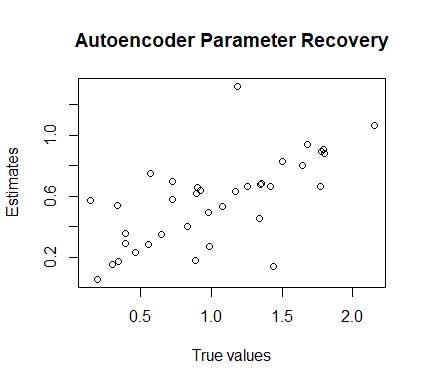
\includegraphics[width=\textwidth]{img/aied_results/ae_a_corr.png}
   \endminipage\hfill
   \minipage{0.5\textwidth}
   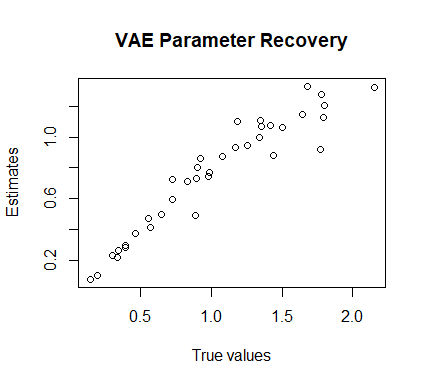
\includegraphics[width=\textwidth]{img/aied_results/vae_a_corr.png}
   \endminipage\hfill
   \caption{Autoencoder and VAE discrimination parameter ($a_{ji}$) recovery.}
   \label{fig:vae_vs_ae_a}
\end{figure}


\begin{figure}[h!]
\minipage{0.5\textwidth}
   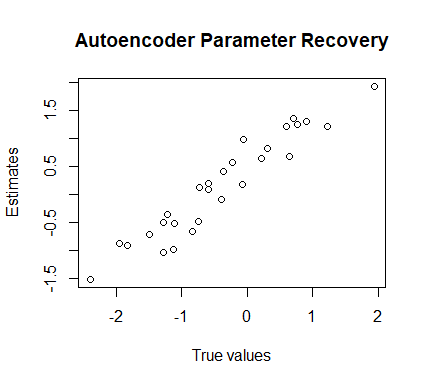
\includegraphics[width=\textwidth]{img/aied_results/ae_b_corr.png}
   \endminipage\hfill
   \minipage{0.5\textwidth}
   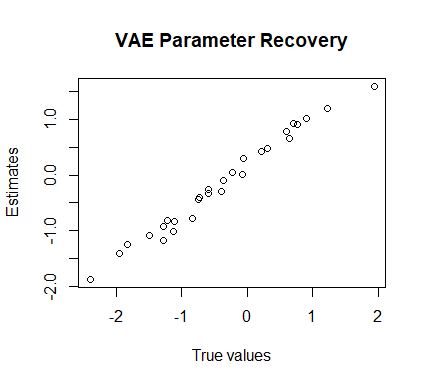
\includegraphics[width=\textwidth]{img/aied_results/vae_b_corr.png}
   \endminipage\hfill
   \caption{Autoencoder and VAE difficulty parameter ($b_i$) recovery.}
   \label{fig:vae_vs_ae_b}
\end{figure}

Results for student ability parameter estimates are shown in Table \ref{tab:vae_vs_ae_theta} and Figure \ref{fig:vae_vs_ae_theta}. Again, we see that the error measures from VAE estimates are much lower than those from AE. However, the correlation values are slightly better for AE, though the difference is not visible in the correlation plot. The reason that AE has poor error measures yes good correlation is because the ability parameter estimates are on a different scale than the true values. Notice in the left plot of Figure \ref{fig:vae_vs_ae_theta} that the vertical axis is on a different scalethan that of the right plot. This is likely due to the fact that a VAE has a KL-divergence term in its loss function.

\begin{table}[h!]
\centering
\begin{tabular}{ccccc}
\hline
Model & $\theta_1$ & $\theta_2$ & $\theta_3$ & Statistic \\
\hline
AE &  7.425 & 3.107 & 16.260 & AVRB \\
VAE   & 1.844 & 1.713 & 4.009 &  \\
\hline
AE & 1.788 & 1.523 & 1.746 & RMSE \\
VAE   & 0.664 & 0.760 & 0.646 & \\
\hline
AE & 0.970 & 0.937 & 0.971 & CORR \\
VAE   & 0.965 & 0.940 & 0.969 & \\
\hline
\end{tabular}
\caption{Statistics for latent trait prediction.}
\label{tab:vae_vs_ae_theta}
\end{table}

The lack of a KL-divergence term in an AE also helps explain the poor discrimination parameter estimates shown in the right plot of Figure \ref{fig:vae_vs_ae_a}. The ML2P model can suffer from an identifiability issue without the assumption that student ability parameters follow some probability distribution \cite{ets2005}. Adding a KL-divergence term in the VAE loss function between the encoder output and the prior $p(\theta)$, which is $\mathcal{N}(0,I)$ in this case.

\begin{figure}[h!]
\minipage{0.5\textwidth}
   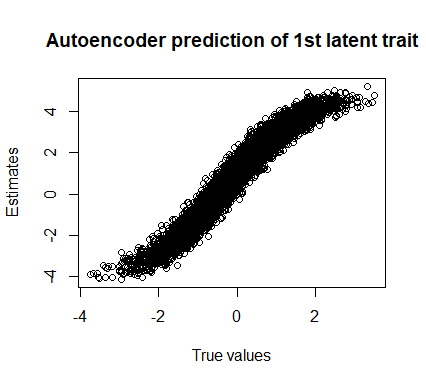
\includegraphics[width=\textwidth]{img/aied_results/ae_theta1_corr.png}
   \endminipage\hfill
   \minipage{0.5\textwidth}
   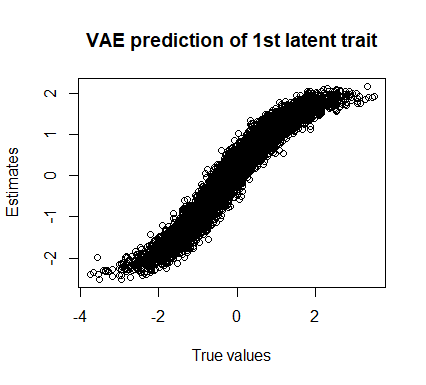
\includegraphics[width=\textwidth]{img/aied_results/vae_theta1_corr.png}
   \endminipage\hfill
   \caption{Autoencoder and VAE predictions for $\theta_1$.}
   \label{fig:vae_vs_ae_theta}
\end{figure}

Both autoencoders and variational autoencoders can be used as IRT parameter estimation methods when a $Q$-matrix restricts weights in the decoder. In either case, adding interpretability to neural networks is interesting, but a VAE is able to incorporate an extra piece of domain knowledge in the prior distribution of $\Theta$, leading to more accurate estimates.


\subsection{ML2P-VAE vs Traditional Methods}
ML
\sideremark{TODO: do 1pl in mirt and VAE}


\begin{sidewaystable}
\footnotesize{
\centering
\begin{tabular}{c|c|ccc|ccc|ccc|c}
    Data Set & Method & $a$.RMSE & $a$.BIAS & $a$.COR & $b$.RMSE & $b$.BIAS & $b$.COR &  $\theta$.RMSE & $\theta$.BIAS & $\theta$.COR & Runtime \\
    \hline
& MHRM & 0.0693 & 0.0319  & 0.9986   & 0.0256 & -0.0021 & 0.9999  & 0.714  & -0.0033  & 0.7006 & 1110s \\ 
(i)& QMCEM & 0.149 & -0.067 & 0.9939 & 0.0376 & -0.002 & 0.9998 & 0.7206 & 0.0023 & 0.6939 & 322s\\
6 abilities& MCEM & 0.1497 & -0.0633 &  0.9936 &  0.0383 & 0.0035 & 0.9997 &  0.7206 & -0.0016 & 0.6938 & 1009s\\
Sim-6& ML2P-VAE$_{full}$ & 0.0705 &  0.0255  & 0.9985   & 0.0471 & -0.0079 & 0.9996  & 0.6649   & -0.0178  & 0.7476 & 343s\\
& ML2P-VAE$_{est}$ & 0.1803 & 0.0871  & 0.9891 &  0.064 & -0.0131 & 0.9993  & 0.7109 &  0.0772  & 0.7082 & 364s \\
& ML2P-VAE$_{ind}$ & 0.1218 & -0.0004 & 0.9944   & 0.0597 & -0.0145 & 0.9994  & 0.7222 &  0.0316  & 0.6928 & 252s\\
\hline 
& MHRM* & 0* & 0*&  1* &  0* &  0* &  1* & 0* & 0* &  1* & 162s \\
(ii)& QMCEM & 0.0159  & 0.0035 & 0.9999 & 0.0067  & -0.0005 & 1   & 0.0111 & 0.0007 & 0.9999 & 192s\\
3 abilities & MCEM & 0.0228 & 0.0148 & 0.9998 & 0.0064  & -0.0008 & 1   & 0.0132 & 0.0026 & 0.9998 & 33s \\
ECPE & ML2P-VAE$_{full}$ & N/A & N/A & N/A & N/A & N/A & N/A & N/A & N/A & N/A & N/A  \\
& ML2P-VAE$_{est}$ & 0.2794 & 0.2152 & 0.9713 & 0.148 & 0.0951  & 0.993 & 0.443 & -0.0628 & 0.8237 & 61s  \\
& ML2P-VAE$_{ind}$ & 0.3208 & 0.2184 & 0.9504 & 0.154 & 0.0872  & 0.9932  & 0.3063 & 0.01 & 0.9017 & 49s \\
\hline
& MHRM & N/A & N/A & N/A & N/A & N/A & N/A & N/A & N/A & N/A & N/A  \\
(iii)& QMCEM & N/A & N/A & N/A & N/A & N/A & N/A & N/A & N/A & N/A & N/A \\
20 abilities & MCEM & N/A & N/A & N/A & N/A & N/A & N/A & N/A & N/A & N/A & N/A  \\
Sim-20 & ML2P-VAE$_{full}$ & 0.078 &  0.0473  & 0.9983  & 0.0608 &  0.0054  & 0.9996  & 0.6145 &  0.0065  & 0.7893 & 1292s \\
& ML2P-VAE$_{est}$ & 0.2992  & -0.1304  & 0.9822  & 0.1655 &  0.1215  & 0.9987  & 0.7364   & -0.0276  & 0.7257 & 961s \\
& ML2P-VAE$_{ind}$ & 0.2043 &   0.0592  & 0.9792  & 0.0958   & -0.0029  & 0.9992  & 0.7054 &  0.0747  & 0.7135 & 850s \\
\hline
\end{tabular}
\caption{Error measures for discrimination ($a$), difficulty ($b$), and ability ($\theta$) parameters from various parameter estimation methods on three different data sets. Note that in the ECPE data set, there are no true values, so MHRM estimates are accepted as true. In Sim-20, only ML2P-VAE methods are capable of estimating such high-dimensional latent traits}
  \label{tab:results}
}
\end{sidewaystable}

%n{sidewaystable}
%\footnotesize{
%\centering
%\begin{tabular}{c|c|ccc|ccc|ccc|c}
%Data Set & Method & $a$.RMSE & $a$.BIAS & $a$.COR & $b$.RMSE & $b$.BIAS & $b$.COR &  $\theta$.RMSE & $\theta$.BIAS & $\theta$.COR & Runtime \\
%\hline
%& MHRM & 0.0693 &  0.0319  & 0.9986   & 0.0256 & -0.0021 & 0.9999  & 0.714  & -0.0033  & 0.7006 & 1110s \\ 
%(i)& QMCEM & 0.149 & -0.067 & 0.9939 & 0.0376 & -0.002 & 0.9998 & 0.7206 & 0.0023 & 0.6939 & 322s\\
%6 abilities& MCEM & 0.1497 & -0.0633 & 0.9936 &  0.0383 & 0.0035 & 0.9997 &  0.7206 & -0.0016 & 0.6938 & 1009s\\
%(Simulated) & ML2P-VAE$_{full}$ & 0.0705 & 0.0255  & 0.9985   & 0.0471 & -0.0079 & 0.9996  & 0.6649   & -0.0178  & 0.7476 & 343s\\
%& ML2P-VAE$_{est}$ & 0.1803 &  0.0871  & 0.9891 &  0.064 & -0.0131 & 0.9993  & 0.7109 &  0.0772  & 0.7082 & 364s \\
%& ML2P-VAE$_{ind}$ & 0.1218 &  -0.0004 & 0.9944   & 0.0597 & -0.0145 & 0.9994  & 0.7222 &  0.0316  & 0.6928 & 252s\\
%\hline 
%& MHRM* & 0* & 0*& 1* &  0* &  0* &  1* & 0* & 0* &  1* & 162s \\
%(ii)& QMCEM & 0.0159 & 0.0035 & 0.9999 & 0.0067  & -0.0005 & 1   & 0.0111 & 0.0007 & 0.9999 & 192s\\
%3 abilities & MCEM & 0.0228  & 0.0148 & 0.9998 & 0.0064  & -0.0008 & 1   & 0.0132 & 0.0026 & 0.9998 & 33s \\
%(ECPE) & ML2P-VAE$_{full}$ & N/A & N/A & N/A & N/A & N/A & N/A & N/A & N/A & N/A & N/A  \\
%& ML2P-VAE$_{est}$ & 0.2794  & 0.2152 & 0.9713 & 0.148 & 0.0951  & 0.993 & 0.443 & -0.0628 & 0.8237 & 61s  \\
%& ML2P-VAE$_{ind}$ & 0.3208  & 0.2184 & 0.9504 & 0.154 & 0.0872  & 0.9932  & 0.3063 & 0.01 & 0.9017 & 49s \\
%\hline
%& MHRM & N/A & N/A & N/A & N/A & N/A & N/A & N/A & N/A & N/A & N/A  \\
%(iii)& QMCEM & N/A & N/A & N/A & N/A & N/A & N/A & N/A & N/A & N/A & N/A \\
%20 abilities & MCEM & N/A & N/A & N/A & N/A & N/A & N/A & N/A & N/A & N/A & N/A  \\
%(Simulated)& ML2P-VAE$_{full}$ & 0.078 &   0.0473  & 0.9983  & 0.0608 &  0.0054  & 0.9996  & 0.6145 &  0.0065  & 0.7893 & 1292s \\
%& ML2P-VAE$_{est}$ & 0.2992   & -0.1304  & 0.9822  & 0.1655 &  0.1215  & 0.9987  & 0.7364   & -0.0276  & 0.7257 & 961s \\
%& ML2P-VAE$_{ind}$ & 0.2043 &  0.0592  & 0.9792  & 0.0958   & -0.0029  & 0.9992  & 0.7054 &  0.0747  & 0.7135 & 850s \\
%\hline
%\end{tabular}
%\caption{Error measures for discrimination ($a$), difficulty ($b$), and ability ($\theta$) parameters from various parameter estimation methods on three different data sets. Note that in data set (ii), there are no true values, so MHRM estimates are accepted as true. In data set (iii), only ML2P-VAE methods are capable of estimating such high-dimensional latent traits}
%\label{tab:results}
%}
%\end{sidewaystable}\section{3-PL Results}
%(maybe)


%Let me add another figure here:
%\begin{center}
%    \bxfigure[!hb]{Another figure\label{fig2}}{
%  \includegraphics[width=0.8\columnwidth]{fig2}
%}
%\end{center}
